\documentclass[11pt, oneside]{article} 
\usepackage{geometry}
\geometry{letterpaper} 
\usepackage{graphicx}
	
\usepackage{amssymb}
\usepackage{amsmath}
\usepackage{parskip}
\usepackage{color}
\usepackage{hyperref}

\graphicspath{{/Users/telliott_admin/Dropbox/Tex/png/}}
% \begin{center} 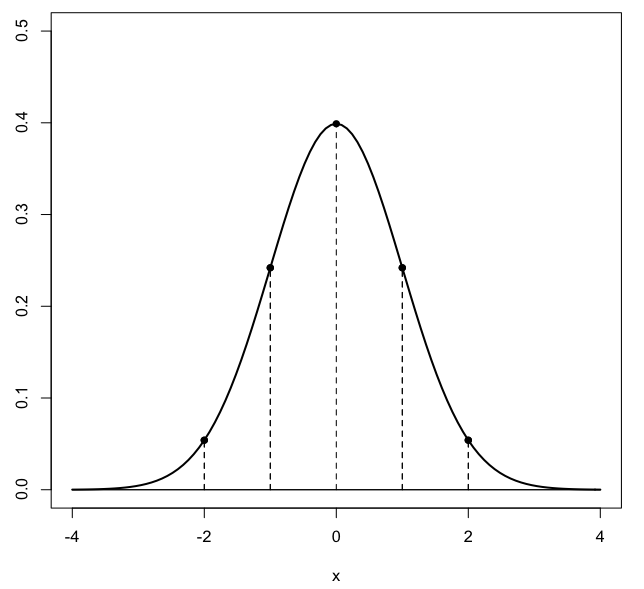
\includegraphics [scale=0.4] {gauss3.png} \end{center}

\title{Hyperbolic substitutions}
\date{}

\begin{document}
\maketitle
\Large

I came across this integral:
\[ \int \sqrt{x^2 - a^2} \ dx \]
with an unusual substitution method to solve it.

We've had $\sqrt{a^2 - x^2}$ as the integrand before, with the circle.  If we manipulate this new expression:
\[ y = \sqrt{x^2 - a^2} \]
\[ y^2 = x^2 - a^2 \]
\[ x^2 - y^2 = a^2 \]
You can see where the hyperbolic connection comes from.  

\subsection*{the answer is}
The best way to solve this is to look it up:
\[ I = \frac{x \sqrt{x^2-a^2}}{2} - \frac{a^2}{2} \ \ln(x + \sqrt{x^2 - a^2}) \]

\url{https://www.quora.com/How-do-you-evaluate-the-integral-int-sqrt-x-2-a-2-dx}

We shouldn't just accept this of course, but check by differentiating.  Make our lives simpler by reserving the factor of $1/2$ from both terms.

We will need
\[ [ \sqrt{x^2 - a^2} \ ]' = \frac{x}{\sqrt{x^2-a^2}} \]

The first term is then
\[  [ x \sqrt{x^2-a^2} \ ]' =  \sqrt{x^2-a^2} + \frac{x^2}{\sqrt{x^2-a^2}} \]
\[ = \frac{2x^2 - a^2}{\sqrt{x^2-a^2}} \]
And the second term is $a^2$ times
\[  [ \ln(x + \sqrt{x^2 - a^2}) \ ]' = \frac{1}{x + \sqrt{x^2 - a^2}} (1 +  \frac{x}{\sqrt{x^2-a^2}} ) \]
\[ = \frac{1}{x + \sqrt{x^2 - a^2}} (\frac{\sqrt{x^2-a^2} + x}{\sqrt{x^2-a^2}} ) \]
\[ = \frac{a^2}{\sqrt{x^2-a^2}} \]
where we have brought back the factor of $a^2$ in the last step.  Subtracting the second term from the first
\[ = \frac{2x^2 - 2a^2}{\sqrt{x^2-a^2}} \] 
\[ = 2 \sqrt{x^2-a^2} \]
and then finally, recall the factor of $1/2$, which yields the desired result.

\subsection*{hyperbolic substitution}
To solve the integral, we use a hyperbolic substitution, which is the interesting part.  It will make the integral trivial, however, getting back to the original variable $x$ will be a challenge.  Let
\[ x = \frac{a}{2} (e^t + e^{-t}) \]

If you look again at the hyperbolic functions, you'll see that this is just $x = a \cosh t$.  Let's work through the substitution:
\[ x^2 = \frac{a^2}{4} \ (e^{2t} + 2 + e^{-2t}) \]
\[ \sqrt{x^2 - a^2} = \sqrt{ \frac{a^2}{4} \ (e^{2t} + 2 + e^{-2t}) - a^2} \]
\[ = \sqrt{ \frac{a^2}{4} \ (e^{2t} - 2 + e^{-2t})} \]
a bit tricky, but it works.
\[ = \frac{a}{2} \ (e^t - e^{-t}) \]
\[ = a \sinh t \]

So that's going to be a big help.  We can get $dx$ by differentiation of $\cosh t$ directly, or work through the exponentials:
\[ x = \frac{a}{2} (e^t + e^{-t}) \]
\[ dx = \frac{a}{2} (e^t - e^{-t}) \ dt = a \sinh t \ dt \]

\subsection*{integral}
So after the substitution, the integral is
\[ \int  a^2 \sinh^2 t \ dt \]
which turns out to be easy in terms of the exponentials
\[ = \int \frac{a^2}{4} \ (e^t - e^{-t})^2 \ dt \]
\[ = \int \frac{a^2}{4} \ (e^{2t} - 2 + e^{-2t}) \ dt \]
\[ = \frac{a^2}{4} \ (\frac{e^{2t}}{2} - 2t - \frac{e^{-2t}}{2} )  \]
That was easy, which is the whole point.

\subsection*{reversing the substitution:  term 2}
This is the tricky part.  We have the integral in terms of $t$.  For a nice value of $x$ we could maybe figure out the new bounds for $t$ but in general we have to go back to $x$.  So
\[ x = \frac{a}{2} (e^t + e^{-t}) \]
Let $e^t = z$ and $t = \ln z$ so
\[ x = \frac{a}{2} (z + \frac{1}{z}) \]
\[ z^2 - \frac{2x}{a} z + 1 = 0 \]
\[ z = \frac{(2x/a) \pm \ \sqrt{(2x/a)^2 - 4}}{2} \]
taking only the positive root
\[ = \frac{x}{a} + \sqrt{(x/a)^2 - 1} \]
\[ = \frac{1}{a} (x + \sqrt{x^2 - a^2}) \]
So
\[ t = \ln z = \ln | x + \sqrt{x^2 - a^2} | - \ln | a | \]

Recall that the solution to the integral had one term with $t$ that we can now write:
\[  - \frac{a^2}{4} \ 2t = - \frac{a^2}{2} \ [ \ \ln | x + \sqrt{x^2 - a^2} | - \ln a \ ] \]
The latter part of this gets folded into the constant of integration so
\[ = - \frac{a^2}{2} \ \ln | x + \sqrt{x^2 - a^2} | + C \]
which matches the second half of the answer we were given.  

\subsection*{reversing the substitution:  term 1}
The other part is
\[ = \frac{a^2}{4} \ (\frac{e^{2t}}{2} - \frac{e^{-2t}}{2} )  \]

We know the answer so let's work backwards from that
\[ x = \frac{a}{2} (e^t + e^{-t}) \]
\[ \sqrt{x^2 - a^2} = \frac{a}{2} \ (e^t - e^{-t}) \]
So
\[ x \ \sqrt{x^2 - a^2} = \frac{a^2}{4} (e^t + e^{-t}) (e^t - e^{-t})  \]
\[ = \frac{a^2}{4} (e^{2t}  - e^{-2t}) \]
Multiply the last expression by $1/2$ and we obtain
\[ = \frac{a^2}{4} \ (\frac{e^{2t}}{2} - \frac{e^{-2t}}{2} )  \]

Therefore this expression is equal to
\[ \frac{1}{2} x \ \sqrt{x^2-a^2} \]
which completes the proof.

$\square$

I put this problem in the book because of the interesting substitution, and to give a little more exposure to the hyperbolic functions.  It is harder than your typical integral.  

I would prefer (with Strang) to just admit that there are a lot of hard integrals that can be solved, and then move on.  We have more interesting things to do with our time.  

It also helps to remember that for real problems, they usually cannot be solved in "closed form," so learning a bunch of integral manipulations is not so helpful in the real world.

\end{document}